% Graphic for TeX using PGF
% Title: C:\Users\CAMUGLIAL_INFO\Desktop\Diplome\Diplome\_Documentation\Diagrammes\PathToGpx
% Creator: Dia v0.97.2
% CreationDate: Fri May 26 09:08:06 2017
% For: admintech
% \usepackage{tikz}
% The following commands are not supported in PSTricks at present
% We define them conditionally, so when they are implemented,
% this pgf file will use them.
\ifx\du\undefined
  \newlength{\du}
\fi
\setlength{\du}{15\unitlength}
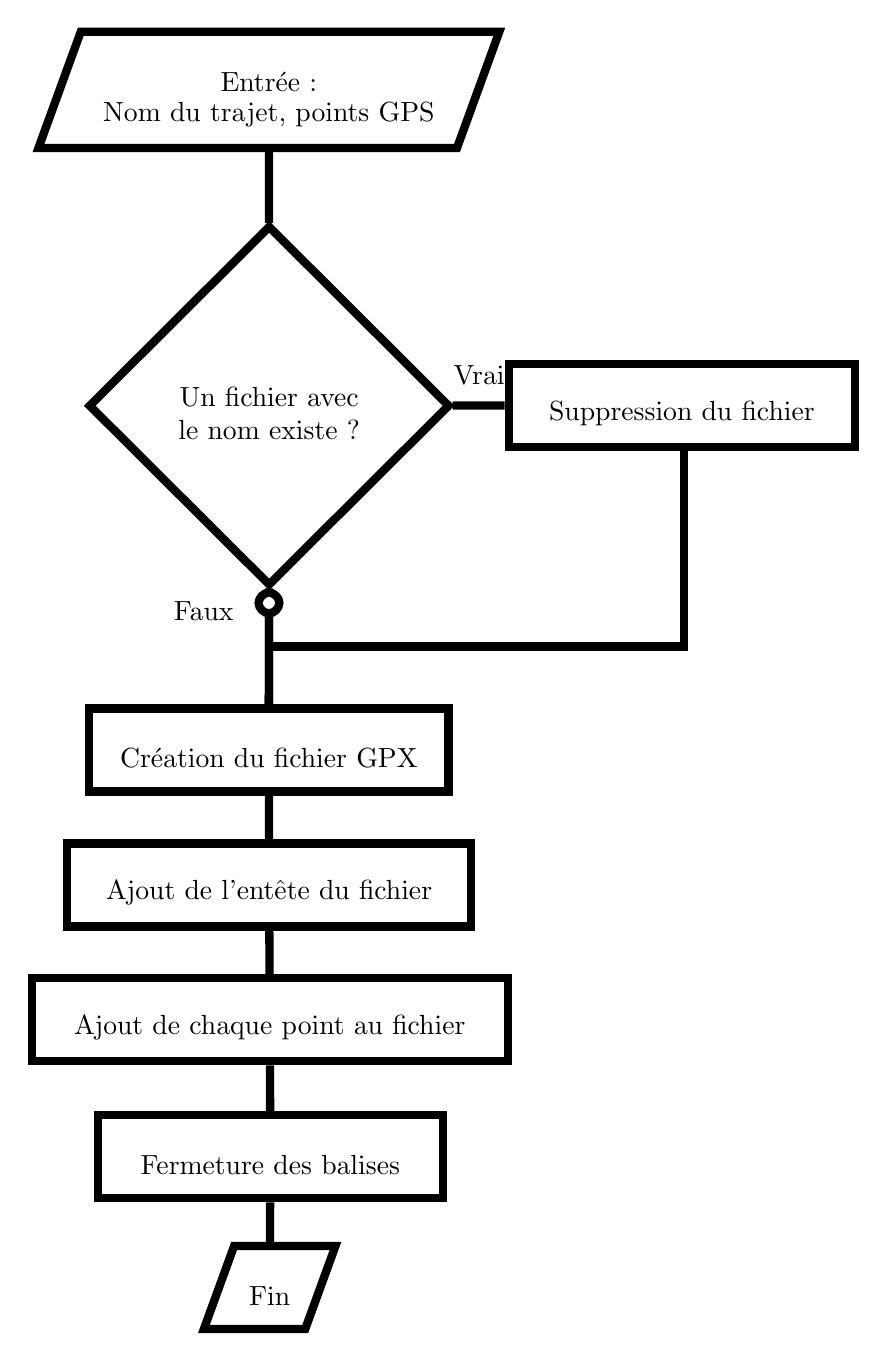
\begin{tikzpicture}
\pgftransformxscale{1.000000}
\pgftransformyscale{-1.000000}
\definecolor{dialinecolor}{rgb}{0.000000, 0.000000, 0.000000}
\pgfsetstrokecolor{dialinecolor}
\definecolor{dialinecolor}{rgb}{1.000000, 1.000000, 1.000000}
\pgfsetfillcolor{dialinecolor}
\definecolor{dialinecolor}{rgb}{1.000000, 1.000000, 1.000000}
\pgfsetfillcolor{dialinecolor}
\fill (19.368382\du,4.400000\du)--(29.450735\du,4.400000\du)--(28.431618\du,7.200000\du)--(18.349265\du,7.200000\du)--cycle;
\pgfsetlinewidth{0.200000\du}
\pgfsetdash{}{0pt}
\pgfsetdash{}{0pt}
\pgfsetmiterjoin
\definecolor{dialinecolor}{rgb}{0.000000, 0.000000, 0.000000}
\pgfsetstrokecolor{dialinecolor}
\draw (19.368382\du,4.400000\du)--(29.450735\du,4.400000\du)--(28.431618\du,7.200000\du)--(18.349265\du,7.200000\du)--cycle;
% setfont left to latex
\definecolor{dialinecolor}{rgb}{0.000000, 0.000000, 0.000000}
\pgfsetstrokecolor{dialinecolor}
\node at (23.900000\du,5.595000\du){Entrée : };
% setfont left to latex
\definecolor{dialinecolor}{rgb}{0.000000, 0.000000, 0.000000}
\pgfsetstrokecolor{dialinecolor}
\node at (23.900000\du,6.395000\du){Nom du trajet, points GPS};
\definecolor{dialinecolor}{rgb}{1.000000, 1.000000, 1.000000}
\pgfsetfillcolor{dialinecolor}
\fill (23.907525\du,9.100000\du)--(28.229730\du,13.406405\du)--(23.907525\du,17.712810\du)--(19.585320\du,13.406405\du)--cycle;
\pgfsetlinewidth{0.200000\du}
\pgfsetdash{}{0pt}
\pgfsetdash{}{0pt}
\pgfsetmiterjoin
\definecolor{dialinecolor}{rgb}{0.000000, 0.000000, 0.000000}
\pgfsetstrokecolor{dialinecolor}
\draw (23.907525\du,9.100000\du)--(28.229730\du,13.406405\du)--(23.907525\du,17.712810\du)--(19.585320\du,13.406405\du)--cycle;
% setfont left to latex
\definecolor{dialinecolor}{rgb}{0.000000, 0.000000, 0.000000}
\pgfsetstrokecolor{dialinecolor}
\node at (23.907525\du,13.201405\du){Un fichier avec};
% setfont left to latex
\definecolor{dialinecolor}{rgb}{0.000000, 0.000000, 0.000000}
\pgfsetstrokecolor{dialinecolor}
\node at (23.907525\du,14.001405\du){le nom existe ?};
\definecolor{dialinecolor}{rgb}{1.000000, 1.000000, 1.000000}
\pgfsetfillcolor{dialinecolor}
\fill (29.681250\du,12.400000\du)--(29.681250\du,14.400000\du)--(38.018750\du,14.400000\du)--(38.018750\du,12.400000\du)--cycle;
\pgfsetlinewidth{0.200000\du}
\pgfsetdash{}{0pt}
\pgfsetdash{}{0pt}
\pgfsetmiterjoin
\definecolor{dialinecolor}{rgb}{0.000000, 0.000000, 0.000000}
\pgfsetstrokecolor{dialinecolor}
\draw (29.681250\du,12.400000\du)--(29.681250\du,14.400000\du)--(38.018750\du,14.400000\du)--(38.018750\du,12.400000\du)--cycle;
% setfont left to latex
\definecolor{dialinecolor}{rgb}{0.000000, 0.000000, 0.000000}
\pgfsetstrokecolor{dialinecolor}
\node at (33.850000\du,13.595000\du){Suppression du fichier};
\definecolor{dialinecolor}{rgb}{1.000000, 1.000000, 1.000000}
\pgfsetfillcolor{dialinecolor}
\fill (19.571250\du,20.700000\du)--(19.571250\du,22.700000\du)--(28.228750\du,22.700000\du)--(28.228750\du,20.700000\du)--cycle;
\pgfsetlinewidth{0.200000\du}
\pgfsetdash{}{0pt}
\pgfsetdash{}{0pt}
\pgfsetmiterjoin
\definecolor{dialinecolor}{rgb}{0.000000, 0.000000, 0.000000}
\pgfsetstrokecolor{dialinecolor}
\draw (19.571250\du,20.700000\du)--(19.571250\du,22.700000\du)--(28.228750\du,22.700000\du)--(28.228750\du,20.700000\du)--cycle;
% setfont left to latex
\definecolor{dialinecolor}{rgb}{0.000000, 0.000000, 0.000000}
\pgfsetstrokecolor{dialinecolor}
\node at (23.900000\du,21.895000\du){Création du fichier GPX};
\definecolor{dialinecolor}{rgb}{1.000000, 1.000000, 1.000000}
\pgfsetfillcolor{dialinecolor}
\fill (19.043005\du,23.950000\du)--(19.043005\du,25.950000\du)--(28.770505\du,25.950000\du)--(28.770505\du,23.950000\du)--cycle;
\pgfsetlinewidth{0.200000\du}
\pgfsetdash{}{0pt}
\pgfsetdash{}{0pt}
\pgfsetmiterjoin
\definecolor{dialinecolor}{rgb}{0.000000, 0.000000, 0.000000}
\pgfsetstrokecolor{dialinecolor}
\draw (19.043005\du,23.950000\du)--(19.043005\du,25.950000\du)--(28.770505\du,25.950000\du)--(28.770505\du,23.950000\du)--cycle;
% setfont left to latex
\definecolor{dialinecolor}{rgb}{0.000000, 0.000000, 0.000000}
\pgfsetstrokecolor{dialinecolor}
\node at (23.906755\du,25.145000\du){Ajout de l'entête du fichier};
\definecolor{dialinecolor}{rgb}{1.000000, 1.000000, 1.000000}
\pgfsetfillcolor{dialinecolor}
\fill (18.190370\du,27.200000\du)--(18.190370\du,29.200000\du)--(29.652870\du,29.200000\du)--(29.652870\du,27.200000\du)--cycle;
\pgfsetlinewidth{0.200000\du}
\pgfsetdash{}{0pt}
\pgfsetdash{}{0pt}
\pgfsetmiterjoin
\definecolor{dialinecolor}{rgb}{0.000000, 0.000000, 0.000000}
\pgfsetstrokecolor{dialinecolor}
\draw (18.190370\du,27.200000\du)--(18.190370\du,29.200000\du)--(29.652870\du,29.200000\du)--(29.652870\du,27.200000\du)--cycle;
% setfont left to latex
\definecolor{dialinecolor}{rgb}{0.000000, 0.000000, 0.000000}
\pgfsetstrokecolor{dialinecolor}
\node at (23.921620\du,28.395000\du){Ajout de chaque point au fichier};
\definecolor{dialinecolor}{rgb}{1.000000, 1.000000, 1.000000}
\pgfsetfillcolor{dialinecolor}
\fill (19.781485\du,30.500000\du)--(19.781485\du,32.500000\du)--(28.091485\du,32.500000\du)--(28.091485\du,30.500000\du)--cycle;
\pgfsetlinewidth{0.200000\du}
\pgfsetdash{}{0pt}
\pgfsetdash{}{0pt}
\pgfsetmiterjoin
\definecolor{dialinecolor}{rgb}{0.000000, 0.000000, 0.000000}
\pgfsetstrokecolor{dialinecolor}
\draw (19.781485\du,30.500000\du)--(19.781485\du,32.500000\du)--(28.091485\du,32.500000\du)--(28.091485\du,30.500000\du)--cycle;
% setfont left to latex
\definecolor{dialinecolor}{rgb}{0.000000, 0.000000, 0.000000}
\pgfsetstrokecolor{dialinecolor}
\node at (23.936485\du,31.695000\du){Fermeture des balises};
\pgfsetlinewidth{0.200000\du}
\pgfsetdash{}{0pt}
\pgfsetdash{}{0pt}
\pgfsetbuttcap
{
\definecolor{dialinecolor}{rgb}{0.000000, 0.000000, 0.000000}
\pgfsetfillcolor{dialinecolor}
% was here!!!
\definecolor{dialinecolor}{rgb}{0.000000, 0.000000, 0.000000}
\pgfsetstrokecolor{dialinecolor}
\draw (23.903531\du,17.808834\du)--(23.900998\du,20.600026\du);
}
\definecolor{dialinecolor}{rgb}{0.000000, 0.000000, 0.000000}
\pgfsetstrokecolor{dialinecolor}
\draw (23.902986\du,18.408834\du)--(23.900998\du,20.600026\du);
\pgfsetlinewidth{0.200000\du}
\pgfsetdash{}{0pt}
\pgfsetmiterjoin
\pgfsetbuttcap
\definecolor{dialinecolor}{rgb}{1.000000, 1.000000, 1.000000}
\pgfsetfillcolor{dialinecolor}
\pgfpathmoveto{\pgfpoint{23.903440\du}{17.908834\du}}
\pgfpathcurveto{\pgfpoint{24.028440\du}{17.908947\du}}{\pgfpoint{24.153326\du}{18.034061\du}}{\pgfpoint{24.153213\du}{18.159061\du}}
\pgfpathcurveto{\pgfpoint{24.153099\du}{18.284061\du}}{\pgfpoint{24.027986\du}{18.408947\du}}{\pgfpoint{23.902986\du}{18.408834\du}}
\pgfpathcurveto{\pgfpoint{23.777986\du}{18.408720\du}}{\pgfpoint{23.653100\du}{18.283607\du}}{\pgfpoint{23.653213\du}{18.158607\du}}
\pgfpathcurveto{\pgfpoint{23.653327\du}{18.033607\du}}{\pgfpoint{23.778440\du}{17.908720\du}}{\pgfpoint{23.903440\du}{17.908834\du}}
\pgfusepath{fill}
\definecolor{dialinecolor}{rgb}{0.000000, 0.000000, 0.000000}
\pgfsetstrokecolor{dialinecolor}
\pgfpathmoveto{\pgfpoint{23.903440\du}{17.908834\du}}
\pgfpathcurveto{\pgfpoint{24.028440\du}{17.908947\du}}{\pgfpoint{24.153326\du}{18.034061\du}}{\pgfpoint{24.153213\du}{18.159061\du}}
\pgfpathcurveto{\pgfpoint{24.153099\du}{18.284061\du}}{\pgfpoint{24.027986\du}{18.408947\du}}{\pgfpoint{23.902986\du}{18.408834\du}}
\pgfpathcurveto{\pgfpoint{23.777986\du}{18.408720\du}}{\pgfpoint{23.653100\du}{18.283607\du}}{\pgfpoint{23.653213\du}{18.158607\du}}
\pgfpathcurveto{\pgfpoint{23.653327\du}{18.033607\du}}{\pgfpoint{23.778440\du}{17.908720\du}}{\pgfpoint{23.903440\du}{17.908834\du}}
\pgfusepath{stroke}
\pgfsetlinewidth{0.200000\du}
\pgfsetdash{}{0pt}
\pgfsetdash{}{0pt}
\pgfsetbuttcap
{
\definecolor{dialinecolor}{rgb}{0.000000, 0.000000, 0.000000}
\pgfsetfillcolor{dialinecolor}
% was here!!!
\definecolor{dialinecolor}{rgb}{0.000000, 0.000000, 0.000000}
\pgfsetstrokecolor{dialinecolor}
\draw (28.326538\du,13.403558\du)--(29.581484\du,13.402750\du);
}
\pgfsetlinewidth{0.200000\du}
\pgfsetdash{}{0pt}
\pgfsetdash{}{0pt}
\pgfsetbuttcap
{
\definecolor{dialinecolor}{rgb}{0.000000, 0.000000, 0.000000}
\pgfsetfillcolor{dialinecolor}
% was here!!!
\definecolor{dialinecolor}{rgb}{0.000000, 0.000000, 0.000000}
\pgfsetstrokecolor{dialinecolor}
\draw (23.901477\du,7.293054\du)--(23.903170\du,9.004310\du);
}
\pgfsetlinewidth{0.200000\du}
\pgfsetdash{}{0pt}
\pgfsetdash{}{0pt}
\pgfsetbuttcap
{
\definecolor{dialinecolor}{rgb}{0.000000, 0.000000, 0.000000}
\pgfsetfillcolor{dialinecolor}
% was here!!!
\definecolor{dialinecolor}{rgb}{0.000000, 0.000000, 0.000000}
\pgfsetstrokecolor{dialinecolor}
\draw (23.902286\du,22.800128\du)--(23.904468\du,23.849872\du);
}
\pgfsetlinewidth{0.200000\du}
\pgfsetdash{}{0pt}
\pgfsetdash{}{0pt}
\pgfsetbuttcap
{
\definecolor{dialinecolor}{rgb}{0.000000, 0.000000, 0.000000}
\pgfsetfillcolor{dialinecolor}
% was here!!!
\definecolor{dialinecolor}{rgb}{0.000000, 0.000000, 0.000000}
\pgfsetstrokecolor{dialinecolor}
\draw (23.911786\du,26.050128\du)--(23.916588\du,27.099872\du);
}
\pgfsetlinewidth{0.200000\du}
\pgfsetdash{}{0pt}
\pgfsetdash{}{0pt}
\pgfsetbuttcap
{
\definecolor{dialinecolor}{rgb}{0.000000, 0.000000, 0.000000}
\pgfsetfillcolor{dialinecolor}
% was here!!!
\definecolor{dialinecolor}{rgb}{0.000000, 0.000000, 0.000000}
\pgfsetstrokecolor{dialinecolor}
\draw (23.926573\du,29.299731\du)--(23.931531\du,30.400269\du);
}
\pgfsetlinewidth{0.200000\du}
\pgfsetdash{}{0pt}
\pgfsetdash{}{0pt}
\pgfsetmiterjoin
\pgfsetbuttcap
{
\definecolor{dialinecolor}{rgb}{0.000000, 0.000000, 0.000000}
\pgfsetfillcolor{dialinecolor}
% was here!!!
{\pgfsetcornersarced{\pgfpoint{0.000000\du}{0.000000\du}}\definecolor{dialinecolor}{rgb}{0.000000, 0.000000, 0.000000}
\pgfsetstrokecolor{dialinecolor}
\draw (33.850000\du,14.400000\du)--(33.900000\du,14.400000\du)--(33.900000\du,19.204430\du)--(23.902264\du,19.204430\du);
}}
\definecolor{dialinecolor}{rgb}{1.000000, 1.000000, 1.000000}
\pgfsetfillcolor{dialinecolor}
\fill (23.063507\du,33.648438\du)--(25.504684\du,33.648438\du)--(24.776743\du,35.648438\du)--(22.335567\du,35.648438\du)--cycle;
\pgfsetlinewidth{0.200000\du}
\pgfsetdash{}{0pt}
\pgfsetdash{}{0pt}
\pgfsetmiterjoin
\definecolor{dialinecolor}{rgb}{0.000000, 0.000000, 0.000000}
\pgfsetstrokecolor{dialinecolor}
\draw (23.063507\du,33.648438\du)--(25.504684\du,33.648438\du)--(24.776743\du,35.648438\du)--(22.335567\du,35.648438\du)--cycle;
% setfont left to latex
\definecolor{dialinecolor}{rgb}{0.000000, 0.000000, 0.000000}
\pgfsetstrokecolor{dialinecolor}
\node at (23.920125\du,34.843438\du){Fin};
\pgfsetlinewidth{0.200000\du}
\pgfsetdash{}{0pt}
\pgfsetdash{}{0pt}
\pgfsetbuttcap
{
\definecolor{dialinecolor}{rgb}{0.000000, 0.000000, 0.000000}
\pgfsetfillcolor{dialinecolor}
% was here!!!
\definecolor{dialinecolor}{rgb}{0.000000, 0.000000, 0.000000}
\pgfsetstrokecolor{dialinecolor}
\draw (23.930781\du,32.597649\du)--(23.925829\du,33.550789\du);
}
% setfont left to latex
\definecolor{dialinecolor}{rgb}{0.000000, 0.000000, 0.000000}
\pgfsetstrokecolor{dialinecolor}
\node[anchor=west] at (21.291742\du,18.356069\du){Faux};
% setfont left to latex
\definecolor{dialinecolor}{rgb}{0.000000, 0.000000, 0.000000}
\pgfsetstrokecolor{dialinecolor}
\node[anchor=west] at (28.031703\du,12.670660\du){Vrai};
\end{tikzpicture}
